%=========================================================================
% main.tex
% Social Vulnerability and Diabetic Retinopathy Progression
% Draft manuscript. Compile with pdflatex (TikZ used for Figure 1).
%=========================================================================
\documentclass[11pt]{article}

\usepackage[margin=1in]{geometry}
\usepackage{setspace}
\usepackage{booktabs}
\usepackage{multirow}
\usepackage{graphicx}
\usepackage{amsmath}
\usepackage{tikz}
\usetikzlibrary{arrows.meta, positioning, shapes.geometric, fit, backgrounds, calc, shapes.misc}
\usepackage[numbers,sort&compress]{natbib}
\usepackage{lineno}
\usepackage{authblk}
\usepackage[hidelinks]{hyperref}

\doublespacing
\linenumbers

\title{\textbf{Social Vulnerability and Progression to Vision-Threatening
Diabetic Retinopathy: A County-Level Analysis of 3,119 United States
Counties, 2021}}

\author[1]{Hannah Becker}
\author[4]{Peter Dunphy}
\author[1]{Nora Fadul}
\author[1]{Rizule Naithani}
\author[1,3]{Laura Green}
\author[2]{Phillip Ma}

\affil[1]{George Washington University School of Medicine and Health Sciences,
Department of Ophthalmology}
\affil[2]{George Washington University, Milken Institute School of Public Health}
\affil[3]{Krieger Eye Institute, Sinai Hospital of Baltimore}
\affil[4]{University of Texas at Austin, Department of Government}

\date{}

\begin{document}
\maketitle

\noindent\textbf{Running head:} Social vulnerability and diabetic retinopathy progression

\noindent\textbf{Keywords:} diabetic retinopathy; vision-threatening diabetic
retinopathy; social vulnerability; disease progression; health services research;
spatial epidemiology

\bigskip

\noindent\textbf{Pr\'ecis:} Among United States adults with diagnosed diabetic
retinopathy, the proportion whose disease had reached a vision-threatening stage
increased with county social vulnerability. The gradient was consistent across
racial and ethnic groups, was not narrower among Medicare-eligible adults, and
persisted after spatial adjustment.

\clearpage

%=========================================================================
\section*{Abstract}
%=========================================================================

\noindent\textbf{Objective:} To determine whether county-level social
vulnerability is associated with the proportion of diagnosed diabetic
retinopathy (DR) that has progressed to a vision-threatening stage, independent
of county demographic composition, eye care supply, and spatial structure.

\noindent\textbf{Design:} Cross-sectional analysis of county-level surveillance
estimates.

\noindent\textbf{Subjects:} Adults with diabetes residing in 3,119 United States
counties and county-equivalents, representing 36.1 million adults with diabetes,
9.53 million with DR, and 1.82 million with vision-threatening DR (VTDR).

\noindent\textbf{Methods:} County estimates of DR and VTDR prevalence among
adults with diabetes were obtained from the Centers for Disease Control and
Prevention Vision and Eye Health Surveillance System (VEHSS) for 2021. Because
VEHSS derives county estimates by post-stratification of national
demographic-specific rates onto local population composition, all models were
estimated \emph{within} county $\times$ race/ethnicity $\times$ age strata with
stratum fixed effects, so that county racial and age composition could not
mechanically contribute to the estimated association. Social vulnerability was
measured with the 2020 CDC/ATSDR Social Vulnerability Index (SVI). Geographic
access was measured as road-network drive time from population-weighted county
centroids to the nearest accredited ophthalmology residency program and to the
nearest county containing any patient-care ophthalmologist. Models were
quasibinomial with VTDR cases as successes and all-stage DR cases as trials.
Residual spatial dependence was addressed with a Leroux conditional
autoregressive model.

\noindent\textbf{Main Outcome Measures:} The VTDR share, defined as
vision-threatening DR cases divided by all-stage DR cases among adults with
diabetes.

\noindent\textbf{Results:} Nationally, 19.1\% of diagnosed DR was
vision-threatening. Within demographic strata, each standard deviation increase
in county social vulnerability was associated with higher odds of
vision-threatening disease among people with DR (odds ratio 1.036, 95\% CI 1.032
to 1.039; $P < 0.001$), corresponding to approximately 0.43 percentage points
per standard deviation. The gradient was consistent across all six race-by-age
strata examined ($\beta$ 0.032 to 0.046). It was no smaller among adults aged 65
to 84, who are near-universally Medicare eligible, than among adults aged 40 to
64 (difference 0.008, $P = 0.16$). The association persisted under a Leroux
conditional autoregressive model with strong residual spatial dependence
($\rho = 0.83$): SVI 0.021 (95\% credible interval 0.012 to 0.029). The gradient
was unchanged by adjustment for Medicare imaging, evaluation and management, and
diagnostic test volume per 1,000 beneficiaries (0.035 to 0.035), arguing against
differential detection, but was attenuated by approximately 42\% by county
mammography screening completion (0.035 to 0.021), implicating general
preventive-screening engagement. County uninsured rate and dual-eligible share
did not explain it. Estimated without stratification, the same association was
0.146, indicating that approximately 76\% of the apparent county-level social
gradient in published VEHSS estimates is attributable to demographic
post-stratification rather than to local variation.

\noindent\textbf{Conclusions:} Among adults who already have diabetic
retinopathy, those living in more socially vulnerable counties are more likely
to have disease at a vision-threatening stage. The gradient is not explained by
demographic composition, is not narrowed by Medicare eligibility or explained by
direct measures of insurance coverage or diagnostic intensity, and is distinct
from the well-described association between social disadvantage and DR
occurrence. A substantial part of it is shared with general preventive-screening
engagement, suggesting that the operative failure is not ophthalmology-specific. Analyses of county-level VEHSS estimates that do not hold
demographic composition fixed will substantially overstate local social
gradients.

\clearpage

%=========================================================================
\section{Introduction}
%=========================================================================

Diabetic retinopathy (DR) remains a leading cause of vision impairment among
adults in the United States.\citep{lundeen2023,aao2024ppp} In 2021, an estimated
9.60 million people were living with DR, representing 26.43\% of individuals
with diabetes, and 1.84 million had vision-threatening DR
(VTDR).\citep{lundeen2023}

The distinction between these two figures is clinically decisive and
analytically underused. Whether a person with diabetes develops any retinopathy
is largely a function of glycemic exposure, diabetes duration, and comorbid
vascular risk. Whether that retinopathy is detected while still mild, or instead
presents as severe non-proliferative disease, proliferative disease, or diabetic
macular edema, is a function of whether the person was screened on schedule and
retained in care.\citep{aao2024ppp,weng2024,jani2017} The first is a question
about disease occurrence; the second is a question about disease progression and
timely detection.

A substantial literature establishes that adverse social determinants of health
are associated with reduced eye care utilization and lower adherence to DR
screening.\citep{chaudhury2024,ravindranath2023,taccheri2023} It is
correspondingly well established that DR is more prevalent in socially
disadvantaged populations. Because that association is largely mediated by the
higher prevalence of diabetes itself in disadvantaged populations, it says
comparatively little about the quality or timeliness of ophthalmic care those
populations receive.

The unresolved question is whether social disadvantage is associated with how
far disease has advanced \emph{among people who already have it}. That quantity,
the share of diagnosed DR that is vision-threatening, is a case-mix measure
rather than a burden measure. It is conditioned on disease, so it is largely
orthogonal to diabetes prevalence, and it speaks directly to the adequacy of
screening and follow-up rather than to the social patterning of diabetes.

Addressing this question with county-level surveillance data requires
confronting a measurement problem that has not, to our knowledge, been addressed
in prior applications of these data. The VEHSS county estimates are constructed
by applying national age-, sex-, and race-specific prevalence rates to each
county's demographic composition, and then adjusting by a county random effect
estimated from Medicare and Medicaid claims.\citep{lundeen2023} A county's
racial and age composition therefore moves its published estimate by
construction. Any analysis relating those estimates to county-level social or
demographic indices, including composite indices such as the Social
Vulnerability Index that contain a racial and ethnic minority status component,
will recover part of the post-stratification machinery rather than a local
epidemiologic signal.

We therefore estimate the association between county social vulnerability and DR
progression entirely within county $\times$ race/ethnicity $\times$ age strata,
so that demographic composition is held fixed by design. We further ask whether
any such gradient is narrowed by near-universal insurance coverage at age 65,
whether it is explained by the supply of eye care providers or by geographic
proximity to ophthalmology training infrastructure, and whether it survives
adjustment for spatial dependence.

Figure~\ref{fig:dag} states the proposed causal pathway and the two
non-causal paths our design is built to block.

%-------------------------------------------------------------------------
\begin{figure}[htbp]
\centering
\resizebox{\textwidth}{!}{%
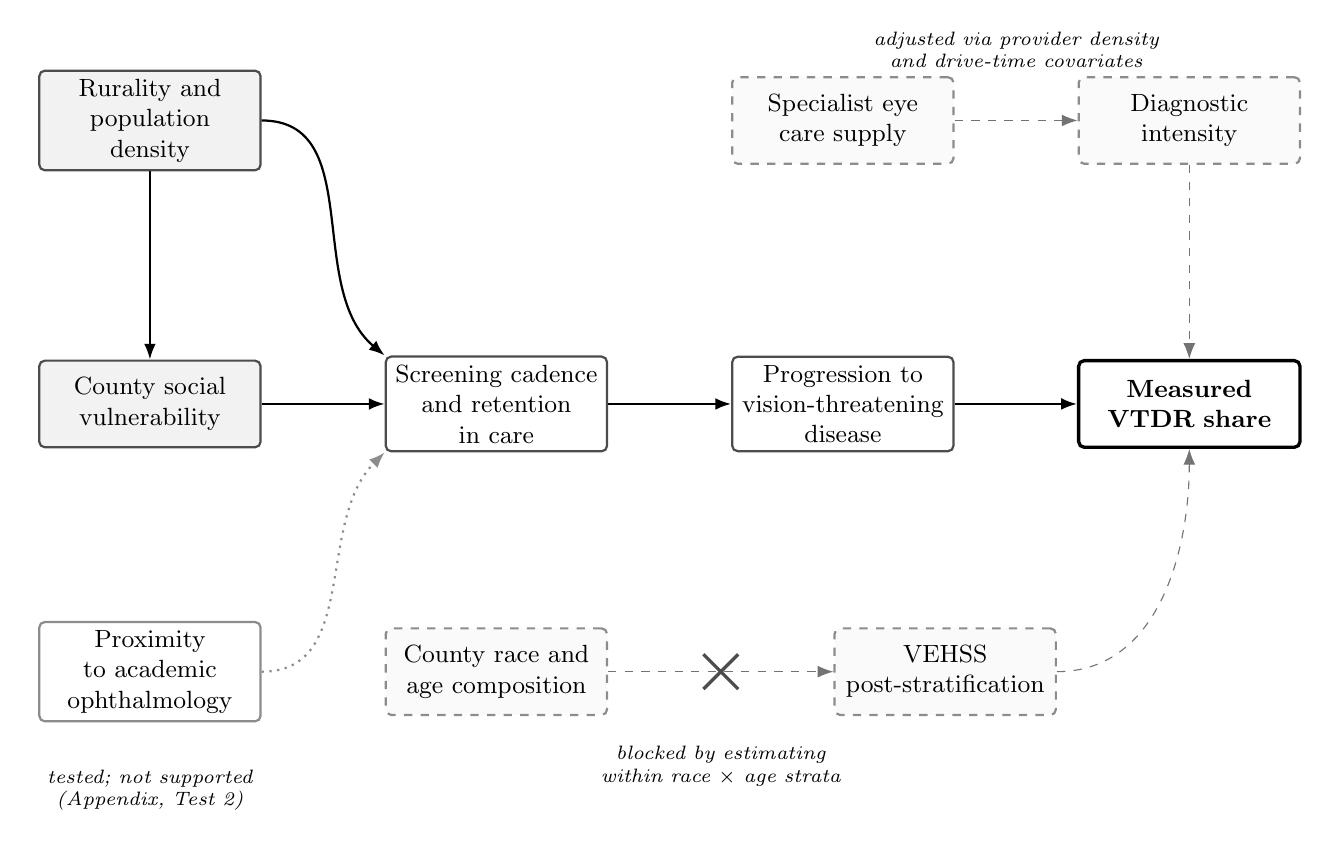
\begin{tikzpicture}[
  x = 1mm, y = 1mm,
  every node/.style = {font=\small},
  box/.style   = {rectangle, rounded corners=2pt, draw=black!70, thick,
                  align=center, inner sep=3pt, minimum height=11mm,
                  text width=26mm, fill=white},
  obs/.style   = {box, fill=black!5},
  outcome/.style = {box, very thick, draw=black},
  bias/.style  = {box, draw=black!45, dashed, fill=black!2},
  null/.style  = {box, draw=black!45, fill=white},
  arr/.style   = {-{Latex[length=2mm]}, thick},
  barr/.style  = {-{Latex[length=2mm]}, dashed, draw=black!55},
  narr/.style  = {-{Latex[length=2mm]}, draw=black!45, dotted, thick},
  lab/.style   = {font=\scriptsize\itshape, align=center, inner sep=1.5pt,
                  fill=white, text width=44mm},
  blocked/.style = {draw=black!70, very thick, cross out, minimum size=4mm,
                    inner sep=0pt}
]

% ---- explicit coordinates keep annotations off the boxes ---------------
% causal chain (y = 0)
\node[obs,     at={(0,0)}]   (svi)  {County social\\vulnerability};
\node[box,     at={(44,0)}]  (scr)  {Screening cadence\\and retention\\in care};
\node[box,     at={(88,0)}]  (prog) {Progression to\\vision-threatening\\disease};
\node[outcome, at={(132,0)}] (meas) {\textbf{Measured}\\\textbf{VTDR share}};

\draw[arr] (svi)  -- (scr);
\draw[arr] (scr)  -- (prog);
\draw[arr] (prog) -- (meas);

% ---- confounder (top left) --------------------------------------------
\node[obs, at={(0,36)}] (rural) {Rurality and\\population density};
\draw[arr] (rural) -- (svi);
\draw[arr] (rural.east) to[out=0, in=140] (scr.north west);

% ---- artifact path 1: differential detection (top right) --------------
\node[bias, at={(88,36)}]  (supply) {Specialist eye\\care supply};
\node[bias, at={(132,36)}] (detect) {Diagnostic\\intensity};
\draw[barr] (supply) -- (detect);
\draw[barr] (detect) -- (meas);
\node[lab, at={(110,45)}] {adjusted via provider density\\and drive-time covariates};

% ---- artifact path 2: post-stratification (bottom) --------------------
\node[bias, at={(44,-34)}]  (comp) {County race and\\age composition};
\node[bias, at={(101,-34)}] (post) {VEHSS\\post-stratification};
\draw[barr] (comp) -- (post);
\draw[barr] (post.east) to[out=0, in=270] (meas.south);
\node[blocked] at (72.5,-34) {};
\node[lab, at={(72.5,-46)}] {blocked by estimating\\within race $\times$ age strata};

% ---- tested but null (bottom left) ------------------------------------
% the posited pathway acts on screening/referral, not on vulnerability itself
\node[null, at={(0,-34)}] (acad) {Proximity to academic\\ophthalmology};
\draw[narr] (acad.east) to[out=0, in=225] (scr.south west);
\node[lab, text width=30mm, at={(0,-49)}] {tested; not supported\\(Appendix, Test 2)};

\end{tikzpicture}}
\caption{Proposed causal pathway from county social vulnerability to the
measured vision-threatening share of diabetic retinopathy. Solid arrows denote
the hypothesized causal chain. Dashed arrows denote non-causal paths that would
induce an association in the absence of any true effect: demographic
post-stratification in the construction of the outcome (blocked by design
through within-stratum estimation) and differential detection driven by
specialist supply (addressed by covariate adjustment). The dotted arrow denotes
the proximity-to-academic-ophthalmology pathway posited in prior work, which we
tested and did not find support for (Appendix, Test~2).}
\label{fig:dag}
\end{figure}
%-------------------------------------------------------------------------

\clearpage

%=========================================================================
\section{Methods}
%=========================================================================

This study follows the STROBE reporting guideline for cross-sectional studies; a
completed checklist is provided as a supplementary file.

\subsection{Study design and setting}

We conducted a cross-sectional analysis of county-level surveillance estimates
for the United States in 2021. All data were publicly available, aggregated, and
contained no individual-level identifiers, so institutional review board
approval was not required.

\subsection{Units of analysis and eligibility}

The unit of analysis was the county or county-equivalent jurisdiction. Of 3,143
counties in the 50 states and the District of Columbia, 3,119 had complete data
on all analytic variables and constituted the analytic sample. Puerto Rico is
not represented in the VEHSS source data and was necessarily excluded.
Connecticut is represented by its eight pre-2022 counties, consistent with the
2021 vintage of all constituent data sources.

\subsection{Outcome}

The primary outcome was the \emph{VTDR share}: the number of people with
vision-threatening DR divided by the number with DR of any stage, among adults
with diabetes. Both quantities were obtained from the CDC Vision and Eye Health
Surveillance System composite prevalence estimates for
2021.\citep{vehss,lundeen2023} VEHSS defines vision-threatening DR as severe
non-proliferative DR, proliferative DR, or diabetic macular edema, and
non-vision-threatening DR as mild to moderate non-proliferative or unspecified
DR without vision-threatening features.\citep{lundeen2023}

We used the published case counts and the corresponding diabetes-population
denominators rather than precomputed rates. Aggregating our county-level
numerators reproduced the published national estimates: DR 26.43\% of adults
with diabetes, VTDR 5.05\%, and a VTDR share of 19.1\%, against published values
of 26.43\%, 5.06\%, and 19.2\% respectively.

\subsection{Handling of post-stratification in the outcome}

VEHSS county estimates are derived by computing national prevalence by age, sex,
and race, applying those rates to each county's population distribution across
the same categories, and adjusting by a county random effect estimated from 2018
Medicaid claims and 2017 to 2019 Medicare Part B fee-for-service
claims.\citep{lundeen2023} County demographic composition therefore enters the
published estimate mechanically.

To remove this pathway, all models were estimated within county $\times$
race/ethnicity $\times$ age cells. We obtained separate VEHSS estimates for
non-Hispanic White, non-Hispanic Black, and Hispanic adults, each in the 40 to
64 and 65 to 84 year age bands, giving six strata and 13,035 analytic cells
across 3,119 counties. Models include stratum fixed effects, so the social
vulnerability coefficient is identified only from differences between counties
within the same race-by-age cell. County demographic composition cannot
contribute to it.

We report the unstratified estimate alongside the stratified estimate to
quantify the magnitude of the artifact.

\subsection{Exposure and covariates}

Social vulnerability was measured using the overall percentile ranking
(\texttt{RPL\_THEMES}) of the 2020 CDC/ATSDR Social Vulnerability
Index,\citep{svi} which is constructed from 2016--2020 American Community Survey
data and uses the same Connecticut county geography as the rest of our data.

Geographic access was characterized by two measures. First, drive time from each
county's population-weighted centroid to the nearest accredited ophthalmology
residency program. Population-weighted centroids were taken from the Census
Bureau's 2020 Centers of Population file,\citep{cenpop} which locates the
centroid where people actually live rather than at the geometric center of the
county polygon. Program locations were compiled from publicly available
FRIEDA/ACGME listings, geocoded, and assigned to counties by point-in-polygon
overlay against 2021 TIGER/Line boundaries; 123 programs accredited in or before
2021, located in 90 counties, were retained. Drive times were computed over the
road network using the Open Source Routing Machine. Second, and to distinguish
academic proximity from eye care availability in general, we computed drive time
to the nearest county containing at least one patient-care ophthalmologist.

Eye care workforce counts were obtained from the Area Health Resources File
2022--2023 release, which carries 2021-vintage counts,\citep{ahrf} and expressed
as patient-care ophthalmologists and optometrists per 100,000 residents. County
population, age structure, and racial and ethnic composition came from the 2021
American Community Survey 5-year estimates. Population density used TIGER/Line
land area, addressing the concern that equally populous counties differing
greatly in area do not carry equal burden density. Rurality was measured with
the 2013 Rural-Urban Continuum Code.

\subsection{External validation data}

Three data systems independent of VEHSS were used to probe the two principal
alternative explanations, differential detection and insurance coverage.

From the CMS Medicare Geographic Variation Public Use File (county level,
2021)\citep{cmsgeo}
we obtained, for the Original Medicare population, imaging events, evaluation
and management events, and diagnostic test events per 1,000 beneficiaries, and
the share of beneficiaries dually eligible for Medicaid. The three utilization
measures index how much diagnostic activity actually occurs in a county, from
claims rather than from provider counts, and are a substantially stronger
control for differential detection than provider density. Dual eligibility
identifies poverty \emph{within} the fully insured 65 and over population.

From County Health Rankings 2021\citep{chr} we obtained the county uninsured rate,
mammography screening completion, influenza vaccination, and preventable
hospital stays (ambulatory-care-sensitive admissions). Mammography completion is
a Medicare-claims measure of whether a county's population follows through on a
recommended preventive screen and has no ophthalmic content; it serves as an
index of general preventive-care engagement. Preventable hospital stays measure
ambulatory care failure in a different organ system and a different data system,
providing a convergent-validity comparison.

Medicaid expansion status as of 2021 was taken from the Kaiser Family Foundation
tabulation.\citep{kff} Twelve states had not adopted expansion; Missouri and Oklahoma
implemented mid-year and were excluded from the expansion contrast rather than
forced into either group. Because expansion altered coverage only for adults
under 65, the 65 to 84 band provides a built-in placebo: any apparent
modification of the social gradient by expansion status that appears equally in
the 65 to 84 band cannot be a coverage effect.

\subsection{Statistical analysis}

Because the outcome is a count of vision-threatening cases out of a count of
total DR cases, we fitted binomial-family generalized linear models with VTDR
cases as successes and all-stage DR cases as trials. County aggregates of this
kind are overdispersed, so all models use the quasibinomial family, which
inflates standard errors by the estimated dispersion rather than treating each
county as an independent Bernoulli sequence.

The primary model regressed the VTDR share on standardized SVI, drive time to
the nearest residency program, drive time to the nearest ophthalmologist,
ophthalmologist and optometrist density, population density, rurality, and
stratum fixed effects. Continuous predictors were standardized, so coefficients
are per standard deviation and directly comparable. Drive times were
log-transformed.

To test whether the gradient reflects insurance coverage, we compared the SVI
coefficient between the 40 to 64 and 65 to 84 age bands within race, using a
two-sample $z$ test on the difference. Medicare eligibility at 65 makes coverage
near-universal in the older band; if the gradient operates through insurance, it
should attenuate there.

Residual spatial autocorrelation was assessed with Moran's $I$ on a queen
contiguity weights matrix. Because dependence was substantial, we refitted the
largest stratum with a Leroux conditional autoregressive spatial random
effect using CARBayes,\citep{carbayes} which accepts binomial counts and trials
directly. Three island counties had no queen neighbor and were linked to their
nearest county so that the adjacency graph was connected. The model was fitted
with a burn-in of 20,000 and 140,000 iterations thinned by 20, yielding 6,000
retained samples; convergence was assessed with Geweke diagnostics (all $|z|<1.3$)
and effective sample sizes (576 to 3,832).

Spearman correlations are reported throughout in preference to Pearson, given
the skewness of county health and workforce distributions.

Analyses were conducted in R version 4.6.0. All data acquisition and analysis
code is publicly available.

\clearpage

%=========================================================================
\section{Results}
%=========================================================================

\subsection{Sample characteristics}

The analytic sample comprised 3,119 counties containing 36.1 million adults with
diabetes, of whom 9.53 million had DR and 1.82 million had vision-threatening
DR. Nationally, 19.1\% of diagnosed DR was vision-threatening, but this share
varied more than fourfold across counties, from 6.9\% to 32.6\%
(interquartile range 14.0\% to 19.2\%).

The VTDR share was essentially uncorrelated with DR prevalence itself
(Spearman $\rho = -0.08$), confirming that disease progression and disease
occurrence are distinct county-level phenomena rather than two expressions of
the same underlying gradient.

Median drive time to the nearest ophthalmology residency program was 123 minutes
(interquartile range 77 to 192). Eighty-eight counties in the analytic sample
contained a program. Notably, 1,950 of 3,119 counties (62.5\%) contained no
patient-care ophthalmologist of any kind.

\subsection{Post-stratification accounts for most of the apparent social gradient}

Estimated without holding demographic composition fixed, each standard deviation
of county social vulnerability was associated with a coefficient of 0.146 on the
log-odds of vision-threatening disease among people with DR. Estimated within
race-by-age strata, the same association was 0.035. Approximately 76\% of the
apparent county-level social gradient in published VEHSS estimates is therefore
attributable to demographic post-stratification rather than to local variation
(Table~\ref{tab:main}).

This has direct implications for the interpretation of prior and future work
using these widely used county estimates, and we return to it in the Discussion.

\subsection{Social vulnerability and disease progression}

Within demographic strata, higher county social vulnerability remained
associated with a greater vision-threatening share of diagnosed DR
(Table~\ref{tab:main}). Each standard deviation increase in SVI corresponded to
an odds ratio of 1.036 (95\% CI 1.032 to 1.039; $P<0.001$), equivalent to
approximately 0.43 percentage points of VTDR share per standard deviation at the
non-Hispanic White 65 to 84 baseline of 14.2\%.

The gradient was strikingly consistent across strata, ranging from 0.032 among
non-Hispanic White adults aged 65 to 84 to 0.046 among Hispanic adults aged 40
to 64, and was statistically significant in every stratum
(Table~\ref{tab:strata}). That the same association appears at similar magnitude
in three racial and ethnic groups and two age bands argues against its being an
artifact of any single population.

\subsection{The gradient is not narrowed by Medicare eligibility}

If the social gradient in disease progression operated principally through
insurance coverage, it should be attenuated among adults aged 65 to 84, for whom
Medicare coverage is near-universal. It was not. The SVI coefficient was 0.150
among adults aged 40 to 64 and 0.142 among adults aged 65 to 84, a difference of
0.008 that did not approach significance ($z = 1.42$, $P = 0.16$; ratio of odds
ratios 1.01). The same pattern held within race strata
(Table~\ref{tab:strata}).

\subsection{Geographic access}

Neither measure of geographic access behaved as an access hypothesis would
predict. In the primary within-stratum model, greater drive time to the nearest
residency program was associated with a \emph{lower}, not higher,
vision-threatening share ($\beta = -0.017$, $P<0.001$), and drive time to the
nearest ophthalmologist was not associated with the outcome
($\beta = -0.002$, $P = 0.52$). Detailed tests of the academic proximity
hypothesis, including capacity-weighted access, discordant-county comparisons,
and university versus community program contrasts, are reported in the Appendix;
none supported it.

\subsection{Spatial confirmation}

Residual spatial dependence was substantial (Moran's $I = 0.237$, $P<0.001$).
Under a Leroux conditional autoregressive model with strong estimated spatial
dependence ($\rho = 0.82$), the social vulnerability association persisted with a
posterior mean of 0.021 (95\% credible interval 0.012 to 0.029). Drive time to
the nearest residency program retained a small negative posterior mean whose
credible interval marginally excluded zero ($-0.010$, 95\% CrI $-0.019$ to
$-0.001$); that is, counties \emph{farther} from a residency program had
slightly \emph{less} vision-threatening disease, the opposite of the direction
an access hypothesis predicts. Optometrist density and rurality also retained
credible intervals excluding zero, while drive time to the nearest
ophthalmologist, ophthalmologist density, and population density did not
(Table~\ref{tab:spatial}).

\subsection{The gradient is unmoved by direct measures of diagnostic intensity}

Adjusting for Medicare imaging, evaluation and management, and diagnostic test
events per 1,000 beneficiaries left the social gradient essentially unchanged
(0.0353 unadjusted to 0.0354 adjusted; Table~\ref{tab:external}). The detection
pathway is nonetheless visible in these data: counties with more Medicare
imaging had a \emph{lower} vision-threatening share
($\beta = -0.028$, $P<0.001$), consistent with greater diagnostic activity
identifying more mild disease. That the social gradient is unaffected by
adjustment for this pathway, while the pathway itself is measurable, is the
strongest evidence available to us that the gradient is not a detection
artifact.

\subsection{General preventive-screening engagement accounts for a substantial share}

Adjusting for county mammography screening completion attenuated the social
gradient from 0.0353 to 0.0206, approximately 42\% on the log-odds scale and
29\% on the standardized scale (Table~\ref{tab:external}). Counties whose
populations completed mammography screening more often had a lower
vision-threatening share of diabetic retinopathy
($\beta = -0.039$, $P<0.001$). Social vulnerability and mammography completion
were correlated at $-0.42$. Influenza vaccination added little beyond
mammography.

\subsection{Direct measures of coverage do not explain the gradient}

Adding the county uninsured rate and the dual-eligible share changed the
gradient only slightly (0.0353 to 0.0343), and neither covariate was
independently associated with the outcome (uninsured $P = 0.14$; dual-eligible
$P = 0.44$). This confirms with direct measures what the age contrast showed
indirectly. Within the 65 to 84 band alone, however, where Medicare coverage is
near-universal, a higher dual-eligible share was still associated with a greater
vision-threatening share ($\beta = 0.006$, $P<0.001$), indicating that poverty
continues to matter after coverage is essentially universal.

\subsection{Medicaid expansion: an apparent effect that the placebo refutes}

The social gradient was roughly three times steeper in expansion states than in
non-expansion states among adults aged 40 to 64 (0.046 vs 0.016). Taken alone
this would suggest expansion modifies the gradient. It does not survive the
placebo. The same contrast appeared, essentially unchanged, among adults aged 65
to 84 (0.042 vs 0.012), an age band whose coverage expansion could not have
altered, and the formal triple interaction was null
(SVI $\times$ expansion $\times$ age band, $\beta = 0.002$, $P = 0.73$;
Table~\ref{tab:expansion}). The apparent difference is therefore state-level
confounding between expansion and non-expansion states rather than a coverage
effect.

\subsection{Convergent validity}

Social vulnerability predicted ambulatory care failure measured entirely outside
VEHSS: each standard deviation was associated with 0.279 standard deviations
more preventable hospital stays ($P<0.001$) and 0.465 standard deviations lower
mammography completion ($P<0.001$). The corresponding standardized association
with the vision-threatening share was 0.100 ($P<0.001$). The diabetic
retinopathy progression gradient is thus real but modest relative to other
county-level care-quality gradients, and sits within a coherent pattern of
social gradients in ambulatory care.

%-------------------------------------------------------------------------
\begin{table}[htbp]
\centering
\caption{Within-stratum model of the vision-threatening share of diabetic
retinopathy, 13,035 county $\times$ race $\times$ age cells across 3,119
counties. Quasibinomial generalized linear model with stratum fixed effects.
Coefficients are per standard deviation on the log-odds scale.}
\label{tab:main}
\begin{tabular}{lrrr}
\toprule
Variable & $\beta$ & SE & $P$ \\
\midrule
Social Vulnerability Index            & $0.0353$  & 0.0016 & $<0.001$ \\
Drive time to residency program (log) & $-0.0174$ & 0.0010 & $<0.001$ \\
Drive time to any ophthalmologist (log)& $-0.0018$ & 0.0028 & $0.52$ \\
Ophthalmologists per 100,000          & $-0.0072$ & 0.0017 & $<0.001$ \\
Optometrists per 100,000              & $-0.0113$ & 0.0023 & $<0.001$ \\
Population density (log)              & $-0.0405$ & 0.0022 & $<0.001$ \\
Rural-Urban Continuum Code            & $-0.0584$ & 0.0032 & $<0.001$ \\
\midrule
\multicolumn{4}{l}{\footnotesize Stratum fixed effects included. Dispersion
parameter 1.93.}\\
\multicolumn{4}{l}{\footnotesize Unstratified comparison estimate for SVI:
$0.146$.}\\
\bottomrule
\end{tabular}
\end{table}
%-------------------------------------------------------------------------

%-------------------------------------------------------------------------
\begin{table}[htbp]
\centering
\caption{Social vulnerability gradient in the vision-threatening share,
estimated separately within each race-by-age stratum.}
\label{tab:strata}
\begin{tabular}{lrrrr}
\toprule
Stratum & $n$ counties & $\beta_{\text{SVI}}$ & SE & $P$ \\
\midrule
Non-Hispanic White, 40--64 & 3,096 & 0.0342 & 0.0030 & $<0.001$ \\
Non-Hispanic White, 65--84 & 3,106 & 0.0320 & 0.0030 & $<0.001$ \\
Non-Hispanic Black, 40--64 & 1,799 & 0.0372 & 0.0049 & $<0.001$ \\
Non-Hispanic Black, 65--84 & 1,533 & 0.0354 & 0.0056 & $<0.001$ \\
Hispanic, 40--64           & 2,060 & 0.0463 & 0.0043 & $<0.001$ \\
Hispanic, 65--84           & 1,441 & 0.0370 & 0.0055 & $<0.001$ \\
\bottomrule
\end{tabular}
\end{table}
%-------------------------------------------------------------------------

%-------------------------------------------------------------------------
\begin{table}[htbp]
\centering
\caption{Leroux conditional autoregressive model, non-Hispanic White adults aged
65 to 84, 3,106 counties. Posterior means and 95\% credible intervals.}
\label{tab:spatial}
\begin{tabular}{lrr}
\toprule
Variable & Posterior mean & 95\% CrI \\
\midrule
Social Vulnerability Index             & $0.0206$  & $0.0115$ to $0.0293$ \\
Drive time to residency program (log)  & $-0.0097$ & $-0.0191$ to $-0.0007$ \\
Drive time to any ophthalmologist (log)& $0.0063$  & $-0.0050$ to $0.0172$ \\
Ophthalmologists per 100,000           & $-0.0031$ & $-0.0126$ to $0.0061$ \\
Optometrists per 100,000               & $-0.0135$ & $-0.0225$ to $-0.0047$ \\
Population density (log)               & $-0.0028$ & $-0.0203$ to $0.0147$ \\
Rural-Urban Continuum Code             & $-0.0201$ & $-0.0324$ to $-0.0072$ \\
\midrule
Spatial dependence $\rho$              & $0.8265$  & $0.7281$ to $0.9112$ \\
\bottomrule
\end{tabular}
\end{table}
%-------------------------------------------------------------------------

%-------------------------------------------------------------------------
\begin{table}[htbp]
\centering
\caption{Social vulnerability coefficient under adjustment for external
measures of diagnostic intensity, preventive-screening engagement, and
insurance coverage. Each block is estimated on its own complete-case sample, so
the base row is repeated for comparability.}
\label{tab:external}
\begin{tabular}{llrrr}
\toprule
Domain & Specification & $\beta_{\mathrm{SVI}}$ & SE & $P$ \\
\midrule
\multirow{2}{*}{Diagnostic intensity}
 & Base (same sample)                 & 0.0353 & 0.0016 & $<0.001$ \\
 & + Medicare imaging, E\&M, tests per 1,000 & 0.0354 & 0.0016 & $<0.001$ \\
\midrule
\multirow{3}{*}{Preventive screening}
 & Base (same sample)                 & 0.0353 & 0.0016 & $<0.001$ \\
 & + Mammography screening            & 0.0206 & 0.0017 & $<0.001$ \\
 & + Mammography and influenza vaccination & 0.0217 & 0.0018 & $<0.001$ \\
\midrule
\multirow{3}{*}{Coverage}
 & Base (same sample)                 & 0.0353 & 0.0016 & $<0.001$ \\
 & + Uninsured rate                   & 0.0335 & 0.0019 & $<0.001$ \\
 & + Uninsured rate and dual-eligible share & 0.0343 & 0.0021 & $<0.001$ \\
\bottomrule
\end{tabular}
\end{table}
%-------------------------------------------------------------------------

%-------------------------------------------------------------------------
\begin{table}[htbp]
\centering
\caption{Medicaid expansion contrast with a built-in placebo. Expansion altered
coverage only for adults under 65, so an equal contrast in the 65 to 84 band
indicates state-level confounding rather than a coverage effect.}
\label{tab:expansion}
\begin{tabular}{llrrr}
\toprule
Age band & Expansion status & Cells & $\beta_{\mathrm{SVI}}$ & SE \\
\midrule
40--64 years & Non-expansion & 2,736 & 0.0163 & 0.0042 \\
40--64 years & Expansion     & 3,822 & 0.0461 & 0.0027 \\
65--84 years & Non-expansion & 2,436 & 0.0122 & 0.0045 \\
65--84 years & Expansion     & 3,307 & 0.0421 & 0.0029 \\
\midrule
\multicolumn{5}{l}{\footnotesize Triple interaction SVI $\times$ expansion
$\times$ age band: $\beta = 0.0023$, $P = 0.73$.}\\
\bottomrule
\end{tabular}
\end{table}
%-------------------------------------------------------------------------

\clearpage

%=========================================================================
\section{Discussion}
%=========================================================================

Among United States adults who already have diabetic retinopathy, those living
in more socially vulnerable counties are more likely to have disease that has
reached a vision-threatening stage. The association is modest in magnitude, on
the order of 0.4 percentage points of VTDR share per standard deviation of
social vulnerability, but it is consistent across racial and ethnic groups and
age bands, is not explained by demographic composition, and survives adjustment
for substantial spatial dependence.

This finding is distinct from the well-established observation that DR is more
prevalent in disadvantaged populations. That association is driven substantially
by the social patterning of diabetes itself. Ours is conditioned on disease: it
concerns how far retinopathy has advanced among those who have it. Because the
progression from mild non-proliferative disease to vision-threatening disease is
the interval in which screening and timely referral operate, a social gradient
in that quantity is more readily interpreted as a gradient in the timeliness and
continuity of ophthalmic care than as a gradient in diabetes risk.

That the gradient is not narrower among Medicare-eligible adults is, in our
view, the most policy-relevant result, and external data reinforce it. Neither
the county uninsured rate nor the dual-eligible share explained the gradient,
and an apparent steepening of the gradient in Medicaid expansion states proved
spurious: the identical contrast appeared among adults aged 65 to 84, whose
coverage expansion could not have altered. Whatever produces this gradient, it
is not principally a coverage mechanism.

Two external tests point instead toward preventive-care engagement. Adjusting
for direct claims measures of diagnostic intensity, Medicare imaging,
evaluation and management, and test volume per 1,000 beneficiaries, left the
gradient completely unchanged, even though those measures are themselves
associated with the outcome in the expected direction. Adjusting for county
mammography screening completion, by contrast, attenuated it by roughly 42\%.
Mammography has no ophthalmic content; what it captures is whether a population
follows through on recommended preventive screening at all. The implication is
that the failure is not ophthalmology-specific but sits in the general
machinery of preventive care, which is consistent with the reported
associations between adverse social determinants and eye care
utilization.\citep{chaudhury2024,ravindranath2023,taccheri2023,liu2018} We note
that mammography is a female-only screen used here as a county-level index, so
it is a marker of screening culture rather than an individual-level mediator,
and this analysis should be read as decomposition rather than formal mediation.

The gradient also sits within a coherent pattern. Social vulnerability predicted
preventable hospital stays, an ambulatory-care-sensitive measure drawn from a
different data system and a different organ system, at 0.279 standard deviations
per standard deviation, against 0.100 for the vision-threatening share. The
diabetic retinopathy result is therefore modest relative to other county care
quality gradients, but it is not anomalous.

We did not find support for the hypothesis that proximity to academic
ophthalmology infrastructure is associated with less advanced disease. If
anything, counties nearer to residency programs showed slightly \emph{higher}
vision-threatening shares, an association that was small but persisted under
spatial adjustment. We interpret this pattern as more likely reflecting diagnostic
intensity than clinical benefit: where subspecialty capacity is concentrated,
vision-threatening disease is more completely identified and coded. This
interpretation is consistent with the caution offered by the authors of the
underlying surveillance estimates, who noted that claims diagnoses are
influenced by access to ophthalmologists and that their model may mistake such
factors for true variation in prevalence.\citep{lundeen2023} A full account of
these tests is given in the Appendix.

Our second contribution is methodological and applies to any study using VEHSS
county estimates. Because those estimates are constructed by post-stratifying
national demographic-specific rates onto local composition, a county's racial
and age structure moves its estimate mechanically. We find that roughly
three-quarters of the apparent county-level social gradient disappears once
demographic composition is held fixed. Analyses that regress these county
estimates on composite social indices, most of which incorporate racial and
ethnic composition, will therefore substantially overstate local social
gradients. We recommend within-stratum estimation as a routine safeguard.

\subsection{Limitations}

First, this is an ecological analysis of county aggregates; associations cannot
be interpreted at the individual level, and the social vulnerability of a county
is not the social circumstance of any patient within it.

Second, and most importantly, the outcome is derived from modeled estimates
built on diagnosed disease in Medicare and Medicaid claims. Disease that is
never diagnosed does not enter. If under-detection is more common in
disadvantaged counties, and if it disproportionately removes mild cases from the
denominator, the VTDR share would rise for reasons unrelated to true
progression. We addressed this with direct claims measures of county diagnostic
intensity rather than provider counts alone, and the gradient was unchanged by
their inclusion, which is reassuring but not dispositive: those measures index
all-cause diagnostic activity rather than retinal screening specifically.
Residual detection bias remains the principal threat, and its likely direction
is to overstate our finding.

Third, VEHSS county random effects were themselves estimated controlling for
ophthalmologists per capita. Including provider density as a covariate is
therefore partly a second adjustment for a factor already partially removed from
the outcome, which will tend to attenuate the estimated role of supply.

Fourth, drive times model private vehicle travel on the road network. They
ignore traffic, are unreliable across ferry routes, and do not represent public
transportation at all. Fourteen island and remote counties in Alaska and Hawaii
had no routable path and are excluded from access analyses.

Fifth, indicator vintages are not perfectly aligned. DR estimates are for 2021,
SVI is constructed from 2016--2020 data, and workforce counts are 2021. The
glaucoma comparison reported in the Appendix is published only for 2022.

Sixth, Puerto Rico is absent from the VEHSS source and is therefore unrepresented
here, as are any counties failing the completeness criteria.

\subsection{Conclusion}

Social vulnerability is associated with more advanced diabetic retinopathy among
people who already have the disease, independent of demographic composition,
provider supply, and spatial structure, and undiminished by Medicare
eligibility. Efforts to reduce preventable vision loss may be better directed at
the timeliness and continuity of retinal screening within disadvantaged
communities than at the geographic placement of academic ophthalmology
infrastructure.

\clearpage

%=========================================================================
\bibliographystyle{plainnat}
\begin{thebibliography}{99}

\bibitem[Ahmed et al.(2025)]{ahmed2025}
Ahmed A, Ali M, Dun C, et al. Geographic distribution of US ophthalmic surgical
subspecialists. \emph{JAMA Ophthalmol.} 2025;143(2):117--124.

\bibitem[American Academy of Ophthalmology(2024)]{aao2024ppp}
American Academy of Ophthalmology. \emph{Diabetic Retinopathy Preferred Practice
Pattern}. 2024.

\bibitem[Berkowitz et al.(2024)]{berkowitz2024}
Berkowitz ST, Finn AP, Parikh R, Kuriyan AE, Patel S. Ophthalmology workforce
projections in the United States, 2020 to 2035. \emph{Ophthalmology.}
2024;131(2):133--139.

\bibitem[Centers for Disease Control and Prevention(2024a)]{vehss}
Centers for Disease Control and Prevention. Vision and Eye Health Surveillance
System: composite prevalence estimates. Available at
\url{https://data.cdc.gov/resource/qeru-k2y2}. Accessed August 2026.

\bibitem[Centers for Disease Control and Prevention(2024b)]{svi}
Centers for Disease Control and Prevention / Agency for Toxic Substances and
Disease Registry. Social Vulnerability Index 2020, county level. Available at
\url{https://svi.cdc.gov}. Accessed August 2026.

\bibitem[Chaudhury et al.(2024)]{chaudhury2024}
Chaudhury AS, Ige M, Marwah S, et al. Race, social determinants of health, and
the quality of diabetic eye care. \emph{JAMA Ophthalmol.}
2024;142(10):961--970.

\bibitem[Feng et al.(2020)]{feng2020}
Feng PW, Ahluwalia A, Feng H, Adelman RA. National trends in the United States
eye care workforce from 1995 to 2017. \emph{Am J Ophthalmol.}
2020;218:128--135.

\bibitem[County Health Rankings(2021)]{chr}
University of Wisconsin Population Health Institute. County Health Rankings \&
Roadmaps 2021 analytic data. Available at
\url{https://www.countyhealthrankings.org}. Accessed August 2026.

\bibitem[Centers for Medicare \& Medicaid Services(2021)]{cmsgeo}
Centers for Medicare \& Medicaid Services. Medicare Geographic Variation by
National, State \& County, 2021. Available at \url{https://data.cms.gov}.
Accessed August 2026.

\bibitem[Kaiser Family Foundation(2021)]{kff}
Kaiser Family Foundation. Status of State Medicaid Expansion Decisions.
Available at \url{https://www.kff.org/medicaid/}. Accessed August 2026.

\bibitem[Health Resources and Services Administration(2023)]{ahrf}
Health Resources and Services Administration. Area Health Resources Files,
2022--2023 release. Available at \url{https://data.hrsa.gov}. Accessed August
2026.

\bibitem[Jani et al.(2017)]{jani2017}
Jani PD, Forbes L, Choudhury A, et al. Evaluation of diabetic retinal screening
and factors for ophthalmology referral in a telemedicine network. \emph{JAMA
Ophthalmol.} 2017;135(7):706--714.

\bibitem[Lee(2013)]{carbayes}
Lee D. CARBayes: an R package for Bayesian spatial modeling with conditional
autoregressive priors. \emph{J Stat Softw.} 2013;55(13):1--24.

\bibitem[Liu et al.(2018)]{liu2018}
Liu Y, Zupan NJ, Shiyanbola OO, et al. Factors influencing patient adherence
with diabetic eye screening in rural communities: a qualitative study.
\emph{PLoS One.} 2018;13(11):e0206742.

\bibitem[Lundeen et al.(2023)]{lundeen2023}
Lundeen EA, Burke-Conte Z, Rein DB, et al. Prevalence of diabetic retinopathy in
the US in 2021. \emph{JAMA Ophthalmol.} 2023;141(8):747--754.

\bibitem[Ravindranath et al.(2023)]{ravindranath2023}
Ravindranath R, Bernstein IA, Fernandez KS, Ludwig CA, Wang SY. Social
determinants of health and perceived barriers to care in diabetic retinopathy
screening. \emph{JAMA Ophthalmol.} 2023;141(12):1161--1171.

\bibitem[Soares et al.(2023)]{soares2023}
Soares RR, Mokhashi N, Sharpe J, et al. Patient accessibility to eye care in the
United States. \emph{Ophthalmology.} 2023;130(4):354--360.

\bibitem[Taccheri et al.(2023)]{taccheri2023}
Taccheri C, Jordan J, Tran D, et al. The impact of social determinants of health
on eye care utilization in a national sample of people with diabetes.
\emph{Ophthalmology.} 2023;130(10):1037--1045.

\bibitem[US Census Bureau(2021)]{cenpop}
US Census Bureau. Centers of Population by County, 2020 Census. Available at
\url{https://www2.census.gov/geo/docs/reference/cenpop2020/}. Accessed August
2026.

\bibitem[Weng et al.(2024)]{weng2024}
Weng CY, Maguire MG, Flaxel CJ, et al. Effectiveness of conventional digital
fundus photography-based teleretinal screening for diabetic retinopathy and
diabetic macular edema: a report by the American Academy of Ophthalmology.
\emph{Ophthalmology.} 2024;131(8):927--942.

\end{thebibliography}

\end{document}
